\documentclass{standalone}
\usepackage{tikz}
\usetikzlibrary{calc}
\begin{document}
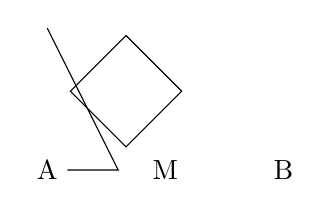
\begin{tikzpicture}
\node (a) at (0,0) {A};
\node (b) at (3,0) {B};
\node at ($(a)!.5!(b)$) {M};
\draw (a) -- ($(a)!0.3!(b)$) -- ($(a)!0.6!90:(b)$);
\draw[rotate around={45:(1,1)}] (0.5,0.5) rectangle (1.5,1.5);
\end{tikzpicture}
\end{document}
